\chapter{Introduction}

\todo{\begin{enumerate}[noitemsep,nolistsep,leftmargin=*]
    \item Molecular structure of DNA (bases, 5'--3', phosphoribose)
    \item DNA copying (strands, complementarity)
    \item Central dogma
    \item Template, coding strand, mRNA, proteins, genetic code
    \item Different polymerases, ncRNA
    \item DNA sequence as string
\end{enumerate}}

\todo{Take intro from paper}

\section{The central dogma}

\begin{figure}[h!]
    \centering
    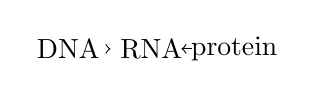
\begin{tikzpicture}
        [every node={circle, draw, inner sep=1em}, node distance=3em]
        \node (dna) {DNA};
        \node (rna) [right of=dna] {RNA};
        \node (protein) [right of=rna] {protein};
        \draw [->] (dna) -- (rna);
        \draw [->] (rna) -- (protein);
    \end{tikzpicture}
    \figcap{dogma}{The central dogma of molecular biology.}{}
\end{figure}

\subsection{Aside: modern modifications to the central dogma and evolution}

\subsection{Transcription}

\subsection{Posttranscriptional modification}

In particular A-to-I conversion (deamination), which is relevant in tRNA gene
wobble base pairing!

\subsection{Translation}

\subsection{The role of \abbr{trna}s in translation}

\section{Gene expression and its regulation}

\section{Using high-throughput sequencing for whole-genome analysis}

\subsection{Explain history and technology of \abbr{hts}}

\section{Types of non-coding \abbr{rna}, their function and expression}

\section{Structure of this thesis}
